\subsection{Oracle}
\subsubsection{Oracle Architektur}


\begin{figure}[ht]
  \centering
  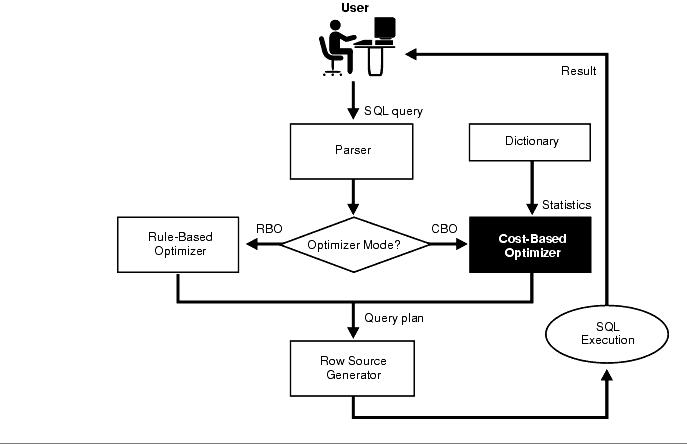
\includegraphics[width=\textwidth]{02_Related_Work/OracleArchitecture.png}
  \caption{Oracle Architecture \cite{Oracle2004Basics}}
  \label{OracleArchitecture}
\end{figure}


Die Oracle Architektur zur Verarbeitung von Anfragen \cite{Oracle2004Basics}  (vgl. Abb. \ref{OracleArchitecture})  beginnt wie die meisten Systeme mit einer SQL Anfrage, die von einem Parser in eine Interne Repräsentation gebracht wird. Der Parser übernimmt dabei zwei Funktionen. Auf der einen Seite die syntaktische Analyse, es wird geprüft, ob die SQL Anfrage die korrekte Syntax besitzt. Auf der anderen Seite eine semantische Analyse, diese prüft beispielsweise ob Datenbank Objekte und Objekt-Attribute  korrekt referenziert werden. 

Ein wesentlicher Unterschiede war bis zu Version 11g der Oracle Datenbank die Verwendung von \ac{RBO} und \ac{CBO}. Je nach Anfrage konnte durch den \ac{DBI} entschieden werden, ob \ac{RBO} bzw. \ac{CBO} zum Einsatz kommt. Mit Version 11g ist diese Möglichkeit weggefallen \cite{dba_oracle2015}. 

Der \ac{QO} führt bei der Verarbeitung die folgenden drei Schritte aus:

\begin{itemize}
\item Eine Menge potenzieller Pläne wird basierend der SQL Anfrage selbst und aufgrund von Hinweisen, die durch den Nutzer eingegeben werden, generiert.

\item Der Optimierer schätzt die Kosten für jeden Plan basierend auf Kosteninformationen über die Anfrage und Storage Charakteristiken der Tabellen, Indexe und Partitionen ,auf die durch ein Statement zugegriffen werden kann.

Die Kostenschätzung für den Zugriff auf entsprechende Datensätze und die Reihenfolge der Joins wird nach ihrem Verbrauch von Ressourcen wie I/O, CPU und Memory geschätzt.

Pläne mit höheren Kosten benötigen mehr Zeit zur Ausführung, als Pläne mit niedrigeren Kosten. Falls Pläne parallel ausgeführt werden können, ist die Ressourcen Nutzung nicht direkt abhängig von der verwendeten Zeit.

\item Der Optimierer vergleicht die Kosten der Pläne und wählt den kostengünstigsten Plan aus.
\end{itemize}

Das Ergebnis des Optimierers ist ein Plan, der zum Ausführen der Anfrage geeignet ist und als kosten-optimal eingeschätzt wird.


\subsubsection{Kostenbasierte Transformation in Oracle}

Traditionelle Relationale Datenbank Systeme führen, wie bereits dargestellt, die Transformation von Anfragen in zwei Phasen durch: Logische und physische Phase. In der logischen Phase wird die gegebene Anfrage zuerst durch einen Rewriter angewendet, hier kommen Heuristiken oder Regeln zum Einsatz. Der traditionelle pyhsische Optimizer arbeitet mit einem einzelnen Query Block aus Restriktionen über Tabellen, Projektionen und Joins. Die physische Optimierungsphase befasst sich mit Access Methoden, Joinreihenfolge und Join Methoden die genutzt werden, um effiziente Pläne zu erzeugen.

Query Transformationen werden entweder als Rewriter Systeme oder als Extention des Plan Generators mit dem pyhsichen Optimierer implementiert. Der erste Ansatz skaliert nicht in komplexen kommerziellen Systemen, der zweite Ansatz ist nur einfach auf ein paar wenige Transformationen anzuwenden. 
Bisher wurden zuerst Rewriter Rules angewendet und dann die Nutzung von Cost Based Trasnformations angewendet. \cite{ahmed2006cost} argumentiert, dass einige Heueristiken nicht immer ein optimales Ergebnis erzeugen und daher mit Hilfe von Cost Based Methoden geprüft werden sollten, bevor sie auf eine Anfrage angewendet werden.


Oracle hat die kostenbasierte Transformation, die logische Transformation und die physische Optimierung kombiniert, um den optimalen Execution Plan zu finden. Der logische Teil des Systems teilt sich in Heueristiken und kostenbasierte Transformationen. Die kostenbasierten Transformationen funktionieren wie folgt:

\begin{itemize}
\item Transformationsalgorithmen konvertieren gesamte Teilanfragebäume in eine sequentiell gleiche Form
\item State Spaces für verschiedene Transformationen
\item State Space Search Algorithmen
\item Möglichkeit zur Deep Copy von Anfrage Böcken und Ihrer Consitutues
\item Cost estimation techique (physical optimizer)
Transformation derective und cost annotations
\end{itemize}

Unterschiedliche Transformationsregeln werden auf unterschiedliche Teile der Anfrage angewendet. So kann beispielsweise die Entschachtelung nur auf verschachtelte Elemente der Anfrage angewendet werden. 
 Während der Optimierung werden die Bäume Bottom up transformiert. Verschiedene Alternativen für eine oder mehrere Transformationen für Elemente in einem Query Tree generieren unterschiedliche States innerhalb des State Space of Transformation. Eine Deep copy wird gemacht, bevor ein bestimmter Status erreicht wird und dessen Kosten durch den Aufruf des physischen Optimierers geschätzt werden. Die Evaluation von jedem States der Transformationsstage, der die besten Kosten bietet wird zurück auf den Ursprungstree angewendet.

Die Oracle Transformationen werden immer hintereinander angewendet. Eine Transformatiosnregel wird immer auf den ganzen Baum angewendet, erst danach folgt die nächste Regel. Die Reihenfolge ist diese: Common sub expression factorization, JPS view merging, join elimination, subquery unnesting, group by distinct view merging, group pruning, predicate move around, set operator factorization, disjunction into union-all exansion, star transfomration and join predicate pushdown. Von dieser Reihenfolge kann jedoch in bestimmten Fällen abgewichen werden. 



\subsubsection{State Space Search Techniques}
Bei der Suche nach einem Plan mit Hilfe von kostenbasierender Transformation stellt sich die grundsätzliche Frage nach einem Trade-off zwischen optimalen Kosten und Execution Kosten. Die Suche nach einer Transformation lohnt sich nur dann, wenn die Kosten für die Suche nach einer besseren Transformation gemeinsam mit der Ausführung der eigentlichen Anfrage geringer sind, als die bisher gefundenen Pläne.

Die Frage nach diesem Problem stellt sich insbesondere, wenn eine große Menge an möglichen alternativen Plänen bestehen. Existieren viele einzelne Objekte einer Anfrage, seien es Query Blocks, Tables join edges predikate, gibt es auch die Möglichkeit, dass viele Regeln auf die Objekte angewendet und somit viele alternative Pläne erzeugt werden können. Wenn $N$ Objekte vorhanden sind und auf diese $N$ Objekte eine Transformation $T$ angewendet wird, dann werden nur durch diese eine Transformation $2^N$ verschiedene Pläne generiert. Diese  Menge wächst weiter, wenn mehrere Transformationen auf die bestehenden Objekte angewendet werden können. 


Um dieses kombinatorische Problem der vielen oin permutationen zu lösen wurden mehrere randomizierte Algorithmen vorgeschlagen. Tabu Search, Genetic Search, Iterative Improvement...

chst mit der Anzahl der Trasnfromationsobjekte. Wenn die Anzahl der Transformationsobjekte klein ist, dann ist eine enumerative Transformationstechnik mit Hilfe Exhaustive search des States vielleicht machbar. Da aber die Anzahl der möglichen Optimierungen mit der Zeit steigt, müssen andere Techniken angewendet werden:


\subsubsection{Join Elimination}
Ein Teil der Optimierung sieht vor, dass Joins eliminiert werden. Ein Grund warum Joins aus einer Anfrage entfernt werden können ist, dass diese nicht notwendig für die Erzeugung des Ergebnisses sind (beispielsweise können durch View Merging Joins obsolet werden.)


%\subsubsection{Filter Predicate Move Around}

%\subsubsection{Group Pruning}
